\chapter{Lab 1: Introduction to WireShark and Layered Protocol}

%\section{WireShark overview}
%List objectives of the lab

The labs for this course were designed to help students better
understand the ideas learned in the classes through hands-on
experiments. 

A better way to understand network protocols is to observe how they
actually work.  A basic tool for observing the messages exchanged
between executing protocol entities is the {\bf packet sniffer}, which
is an essential part of {\bf network protocol analyzer}.  WireShark is
a free and open-source network protocol analyzer that runs on various
operating systems including Linux, Unix, Mac, and Windows. We will
give a brief overview of it in the following section.

This lab has three parts. The first part includes simple tasks that let
you get familiar with the basic operations of WireShark. The second
part will introduce some handy networking tools, which will be used in
the following labs. 
The third part will focus on how protocols and layering are represented 
in packets by exploring the sniffed packet traces.


\section{Overview}

\subsection{WireShark}

WireShark (previously called Ethereal) is one of the most widely used
network protocol analyzer. It passively sniffs packets that are sent
from or received by a designated network interface, but never sends
packets itself. It receives a {\em copy} of packets that are sent from
or received by the applications and protocols executing on the end-system
(e.g., your computer).
%Similarly, received packets are not explicitly addressed to the packet
%sniffer; instead, the sniffer receives a copy of packets that are sent
%from or received by applications and protocols executing on your
%computer.  
WireShark also has a graphical front-end to display the packets that
it sniffs.

\begin{figure}[h]
\centering
 \includegraphics[width=0.8\columnwidth]{figs/lab_1_packetsniffer.eps}
  \caption{Network protocol analyzer structure}\label{packetsniffer}
\end{figure}

Fig.~\ref{packetsniffer}~\cite{umass} shows the structure of a network
protocol analyzer. At the right of the figure shows the protocol stack
and applications (such as a web browser or an FTP client) that normally
run on your computer. The network protocol analyzer, shown within the
dashed rectangle, has two parts, the packet capture and the packet
analyzer.  The packet capture library receives a copy of every
link-layer frame that is sent from or received by a designated network
interface.  Recall that messages exchanged by higher layer protocols
such as HTTP, FTP, TCP, UDP, DNS, or IP all are eventually
encapsulated in link-layer frames that are transmitted over physical
media such as an Ethernet cable. In Fig.~\ref{packetsniffer}, the
assumed physical media is an Ethernet, and so all upper layer
protocols' headers are eventually encapsulated within an Ethernet frame.
Capturing all link-layer frames thus gives you all messages sent from
or received by all protocols and applications executing in your
computer.

The second component is the packet analyzer,
which displays the contents of all fields within a link-layer frame.
In order to do so, the packet analyzer must {\em understand} the
structure of messages exchanged by the protocols. For example,
 we are interested in displaying the various fields in
messages exchanged by the HTTP protocol in Fig.~\ref{packetsniffer}.
The packet analyzer understands the format of Ethernet frames, and
so it can identify the IP datagram within an Ethernet frame. It also
understands the IP datagram format, so it can extract the TCP
segment within the IP datagram. It understands the TCP
segment structure, so it can extract the HTTP message contained in
the TCP segment. Finally, it understands the HTTP protocol and so,
for example, knows that an HTTP message may
contain the string of ``GET'', ``POST'', or ``HEAD''.

\subsection{Networking Tools}

\subsubsection{ping}
\par The {\em ping} program in the source host sends a packet to the
target IP address; if the target is alive, the {\em ping} program in
the target host responds by sending a packet back to the source host.
% As you might have guessed (given that this lab is about ICMP),
Both of these {\em ping} packets carry ICMP messages. Try ``ping -\--help'' to find out its usage.

\subsubsection{ifconfig}
\par The {\em ifconfig} is a tool to configure a network interface, for instance, setting an interface's IP address and netmask,  disabling or enabling a given interface. Try ``ifconfig -\--help'' to find  out its usage.

\subsubsection{netstat}
\par The {\em netstat} is a tool that displays network connections, routing tables, and network interface statistics. It is used for finding problems in the network and to determine the amount of traffic on the network as a performance measurement. Try ``netstat -\--help'' to find its usage.

\subsubsection{wget}
wget is a command-line program that let you fetch a URL. Unlike a web browser, which fetches and executes the entire pages, wget give you the control over exactly which URLs you fetch and when you fetch them. wget has many options (try ``wget -\--help'' to see them) but a URL can be fetched simply with ``wget URL''.

\subsection{Layered Protocol}

Two reference models are used to describe the network architecture, the OSI/ISO reference model and the TCP/IP reference model. The OSI/ISO model divides the network into seven layers and the TCP/IP model divides the network into four layers. No matter which model is used, the basic principle of the layered architecture is that each layer performs some services for the layer above it.

\section{Procedures}
%List procedures of the lab

\subsection{Installation}
WireShark is free to download at http://www.wireshark.org/. How to
build and install WireShark onto machines with different operating
systems can be referred to
http://wiki.wireshark.org/BuildingAndInstalling.


\subsection{Getting familiar with WireShark}
\subsubsection{A. Starting WireShark}
\begin{figure}[!t]
\centering
 \includegraphics[width=0.99\columnwidth]{figs/lab_1_fig_1.eps}
  \caption{WireShark graphical user interface}\label{lab_1_fig_1}
\end{figure}

When you run WireShark, you will see the graphical user interface (GUI) as
shown in Fig.~\ref{lab_1_fig_1}. There are four main fields:
\begin{itemize}
\item \textbf{Filter field}: Used to filter out uninteresting packets
  with the entered specifications, so you can choose which packets
  should (not) be shown on the screen;
\item \textbf{Captured packets}: Lists the packets captured by the
  selected interface;
\item \textbf{Details of selected packet}: Lists information about the
  packet that is selected in the captured packets window;
\item \textbf{Content of packet in hex/ASCII}: Displays the content of
  the captured packet, in hex and ASCII.
\end{itemize}

\subsubsection{B. Capture Trace}

Use the following procedure to capture the trace.

\begin{itemize}
\item Pick a URL and fetch it by {\em wget}. For example, \textbf{open a console}, type ``wget http://www.google.ca'', you will obtain the fetched resource written in a file. A successful example is shown in Fig.~\ref{lab_1_wget_url}. The expected response is ``200 OK''. 


\begin{figure}[!t]
\centering
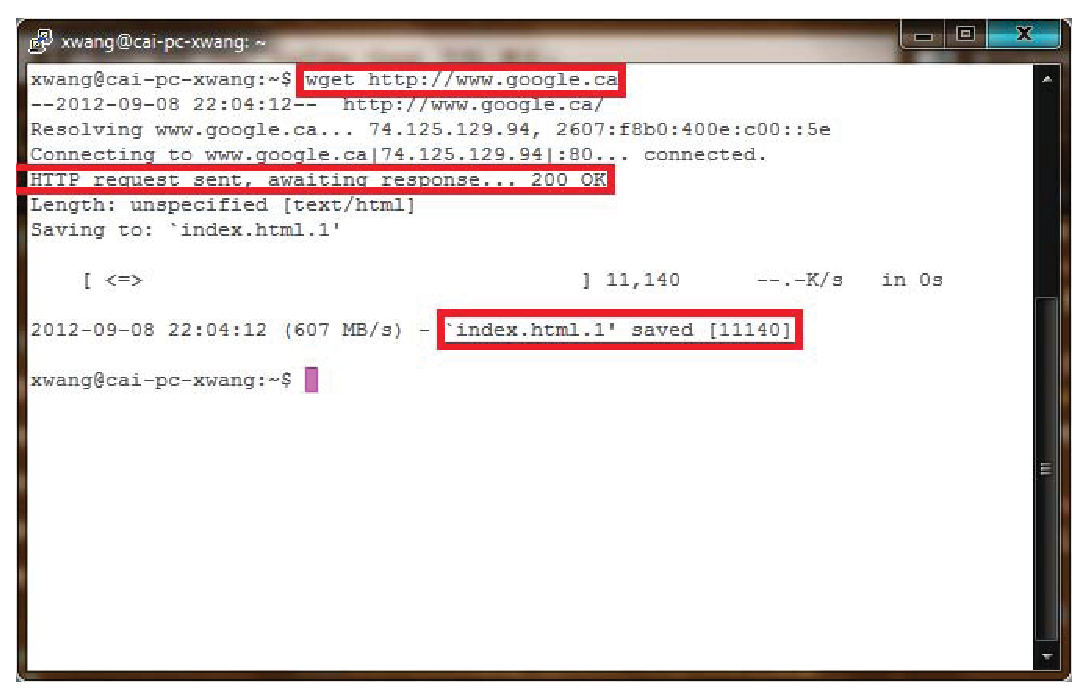
\includegraphics[width=0.8\columnwidth]{figs/lab_1_wget_url.eps}
\caption{Wget URL}\label{lab_1_wget_url}
\end{figure}

\item Close web browser. By minimizing browser activity you will stop your computer from fetching unnecessary web content, and avoid incidental traffic in the trace.

\item Launch Wireshark. Choose the network interface that we would
  like to capture the packets on. To do this, select ``Capture
  $\Rightarrow$ Options'' from the command menu. A window similar to
  the one shown in Fig.~\ref{lab_1_fig_2} should pop up. Select the
  interface you are using. Uncheck ``Capture packets in promiscuous 
  mode''. This mode is useful to overhear packets sent to/from other 
  computers on broadcast networks. We only want to record packets 
  sent to/from your computer. Use capture filter ``tcp port 80''. 
  This filter will record only standard web traffic and not other 
  kinds of packets that your computer may send. Click ``Start'' to 
  start the packet capture process.
 
\begin{figure}[!t]
\centering
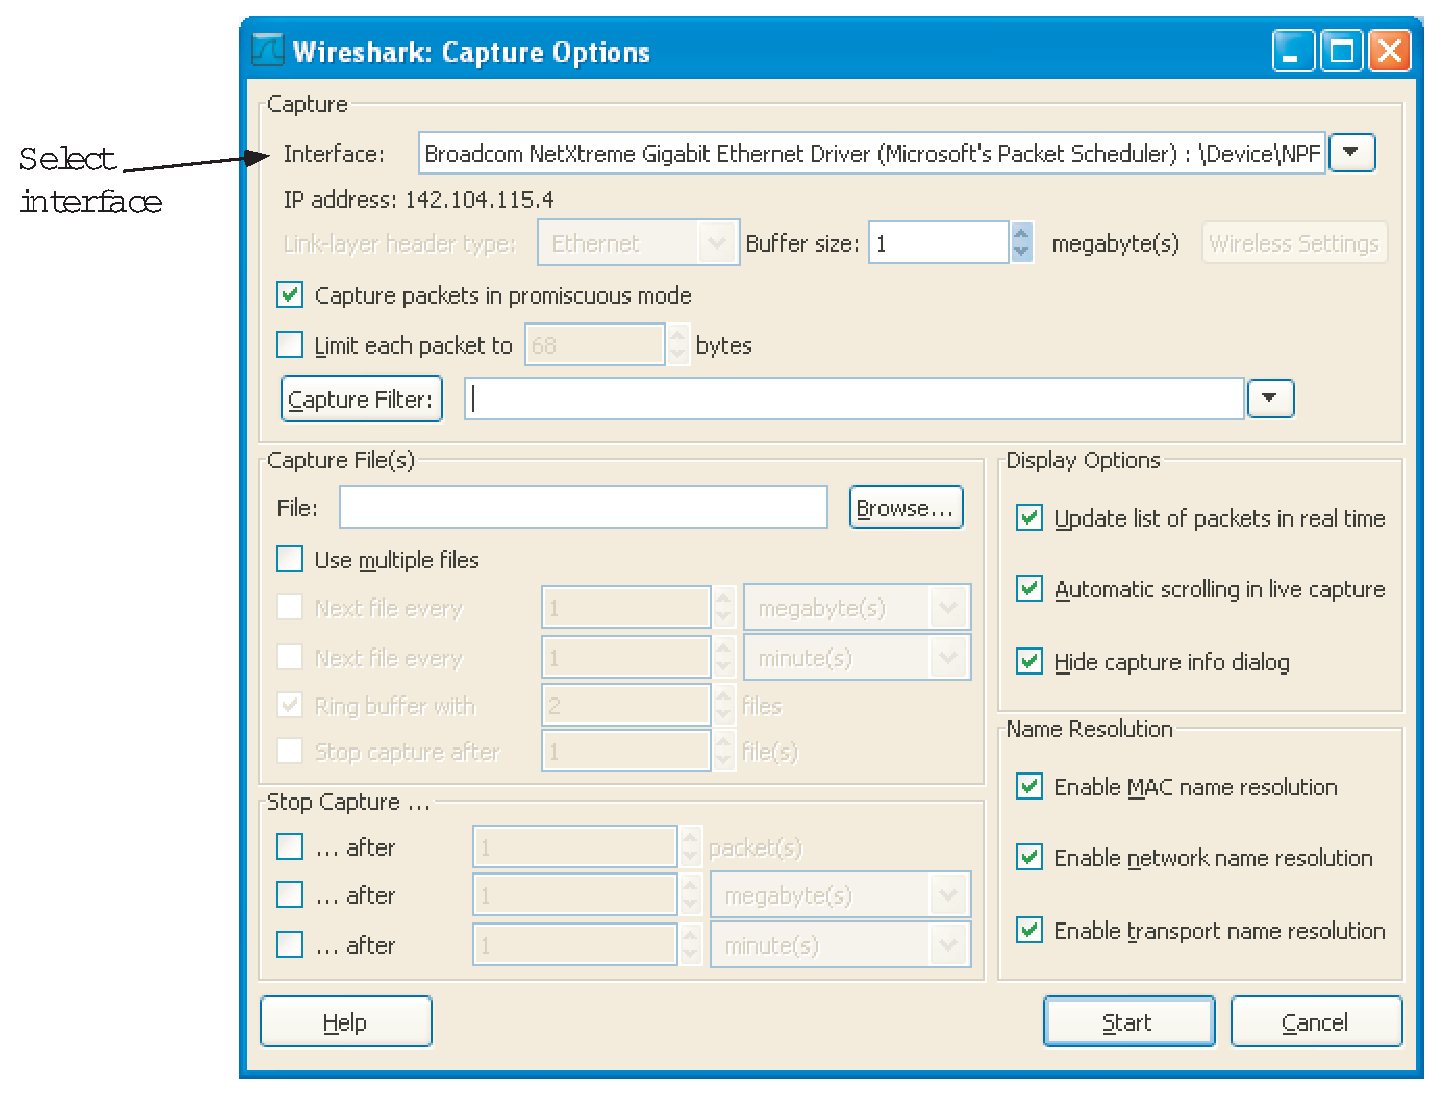
\includegraphics[width=0.8\columnwidth]{figs/lab_1_fig_2.eps}
\caption{Capture options window}\label{lab_1_fig_2}
\end{figure}

\item When the capture is started, repeat the web fetch using wget above. This time, the packets will be recorded by Wireshark as the content is transferred.

\item After the fetch is successful, return to Wireshark and use the menus or buttons to stop the trace (``Capture $\Rightarrow$ Stop''). If you have succeeded, the upper Wireshark window will show multiple packets. How many packets being captured will depend on the size of the web page, but there should be at least 8 packets in the trace. An example is shown in Fig.~\ref{lab_1_wget_wireshark}.

\begin{figure}[!t]
\centering
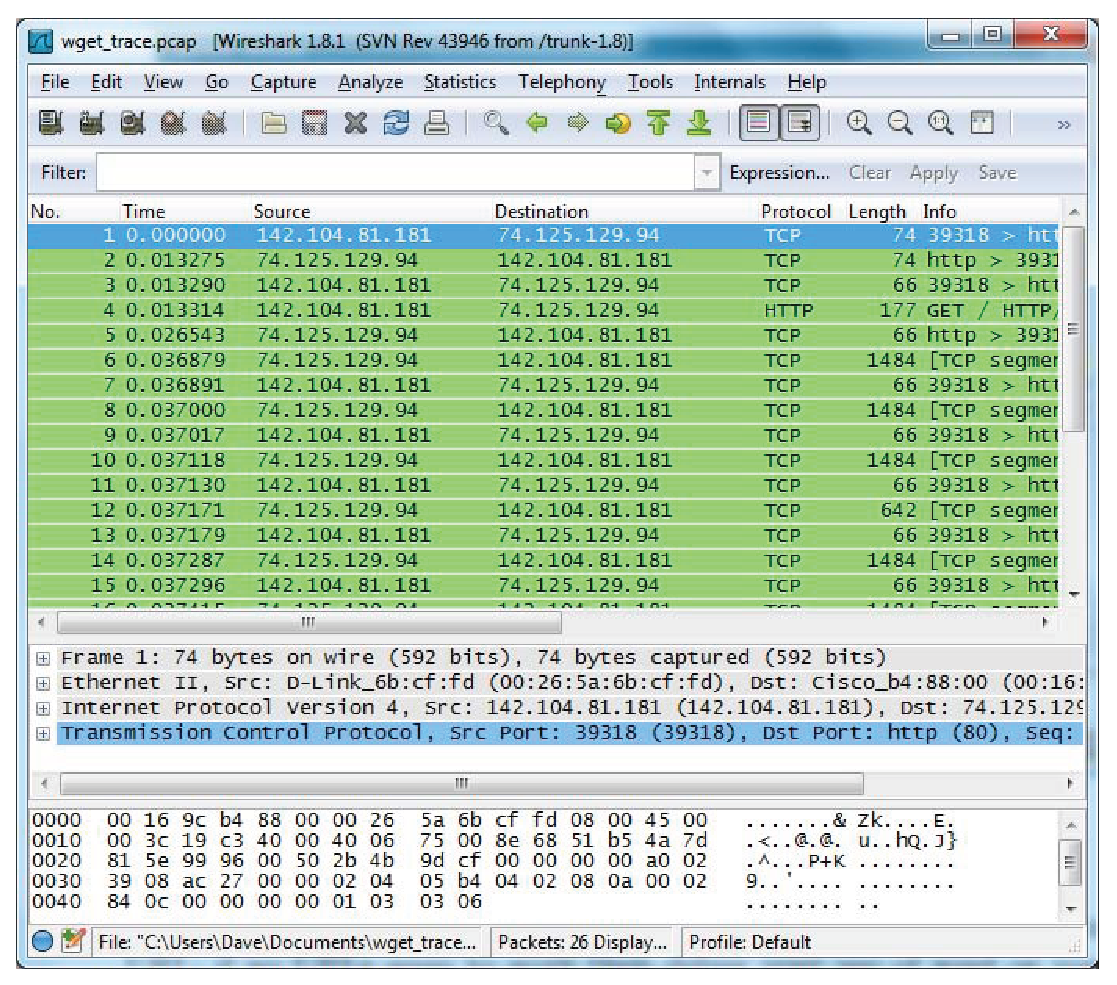
\includegraphics[width=0.8\columnwidth]{figs/lab_1_wget_wireshark.eps}
\caption{Packet trace}\label{lab_1_wget_wireshark}
\end{figure}

\end{itemize}

%\subsubsection{C.  Using traces}


\subsection{Layered Protocol}

%WireShark enables us to create and use traces. Traces are a set of
%captured packets that are saved in a file. In the following few
%experiments, we will use the existing traces to study how the HTTP
%protocol works.

By inspecting the captured trace, or the provided trace ({\bf lab1-wget-trace.pacp}) to understand the layered protocol.


\begin{itemize}
\item Select an HTTP GET packet. This packet carries the HTTP request sent
   from your computer to the server. 
   
\item The protocol layers being used in web fetching are shown in 
 Fig.~\ref{lab_1_protocol_stack_web}. HTTP is the application
 layer web protocol used to fetch URLs. It runs on top of the TCP/IP
  transport and network layer protocols. The link layer protocol shown in the 
  figure is Ethernet. It may be other protocol, depends on your network.   
  
\begin{figure}[!t]
\centering
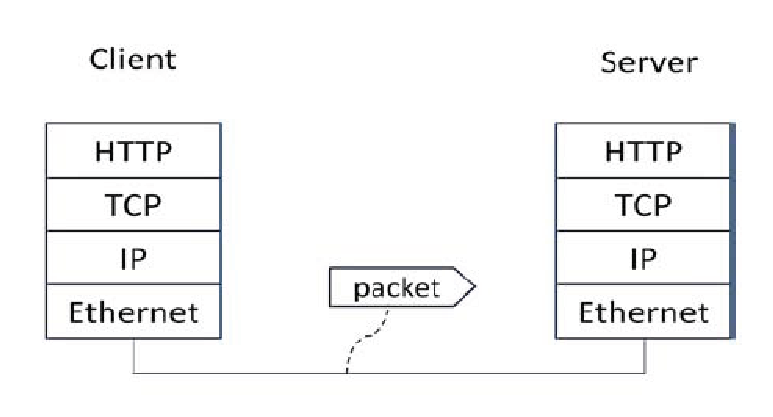
\includegraphics[width=0.8\columnwidth]{figs/lab_1_protocol_stack_web.eps}
\caption{Protocol stack for a web fetch}\label{lab_1_protocol_stack_web}
\end{figure}

\item Click on one HTTP packet, and turn to the middle panel with details of the packet. The first block is ``Frame''. This is a record that describes overall information about the packet, including when it was captured and how many bits long it is. The second block is ``Ethernet'' (You may have taken trace in a computer with 802.11, but still you will see an Ethernet block. This is because Wireshark capture traffic in Ethernet format determined on the capture options. See Link-layer header type.). Then we can see IP, TCP, and HTTP. This is a bottom-up order, because as packets are passed down the protocol stack, the header of the lower layer protocol is added to the front of the information from the higher layer protocol. That is, the lower layer protocols come first in the packet.

\item When an Ethernet frame arrives at a computer, the Ethernet layer must hand the packet that it contains to the next higher layer to be processed. In order to do this, the protocol use information in its header to determine the higher layer data unit encapsulated. Which field is used here?

\item Draw a figure of an HTTP GET packet that shows the position and size in bytes of the TCP, IP and Ethernet protocol headers. On this drawing, show the range of header and payload of each layer. 

\end{itemize}
 
\section{Discussion}

\subsection{Running WireShark}
\label{Dis_run_wireshark}

\begin{enumerate}

\item Capture a trace without filter.

\item List at least 3 different protocols that appear in the protocol
  column in the {\em unfiltered} packet-listing window.

\item How long did it take from the HTTP GET message being sent
  to the HTTP OK reply being received?

\end{enumerate}

\subsection{Networking Tools}

Explore the usage of ``ifconfig'', ``ping'', ``netstat'', and answer the following questions. (\textbf{Hint:} If you're not sure about how to use these commands, please check \textsl{Sec.~1.1.2 Networking Tools"}.)

\begin{enumerate}

\item  How many Ethernet interfaces are in your computer, how to determine it?

\item How to turn down/up an Ethernet interface?

\item Ping 10 packets to two websites. Compare the statistic results (packet loss, avg rtt).

\end{enumerate}

\subsection{Layered Protocol}

\begin{enumerate}

\item Draw the structure of a HTTP GET packet.

\item In the provided trace ({\bf lab1-wget-trace.pacp}), calculate the average overhead of \textbf{all} the packets \textbf{from the server to the client} (in percentage). ({\bf Hint:} For one packet, the overhead is the size of all headers in one packet over the total size. The average overhead is the ratio between total size of headers and total size of the packets).

\item Which Ethernet header field tells the next higher layer protocol is IP? What value it used?

\item Which IP header field tells the next higher layer protocol is TCP? What value it used?
\end{enumerate}

%\begin{thebibliography}{99}
%\bibitem{umass}Ethereal Labs,
%  http://www-net.cs.umass.edu/ethereal-labs
%\bibitem{wiki}Wikipedia.org,
%  http://en.wikipedia.org/wiki/HTTP
%\end{thebibliography}
